\begin{figure}[!ht]
    \centering
    % \includegraphics{}
    a)
    \begin{minipage}{.45\textwidth}
        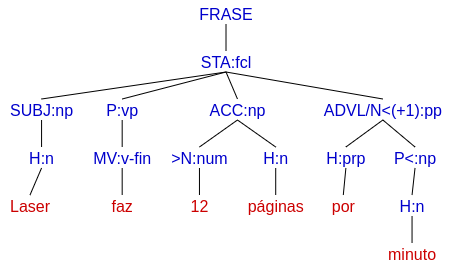
\includegraphics[width=\linewidth]{imagens/ec_bosque_sem_ponto_tree_orig.png}
        \caption{árvore original};
    \end{minipage}
    % 
    b)
    \begin{minipage}{.45\textwidth}
        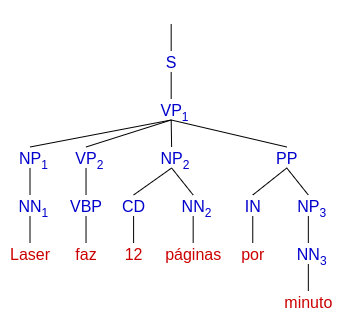
\includegraphics[width=\linewidth]{imagens/ec_bosque_sem_ponto_tree_trans.png}
        \caption{árvore transduzid;a}
    \end{minipage}
    c)
    \begin{minipage}{.45\textwidth}
        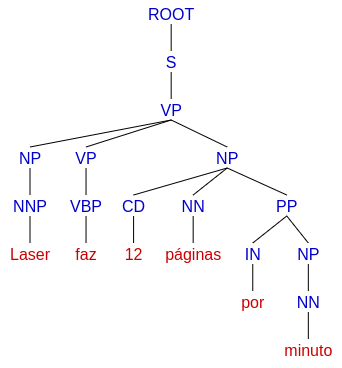
\includegraphics[width=\linewidth]{imagens/ec_bosque_sem_ponto_tree_sp.png}
        \caption{árvore gerada pelo; SP}
    \end{minipage}
    \caption[Estudo de caso BOSQUE - Sentença transduzida sem pontuação]{Estudo da sentença CF761-1, \textquote{Laser faz 12 páginas por minuto}, que originalmente não possui nenhuma pontuação. Em a), vemos a árvore relativa à sentença original no BOSQUE. Em b), a sentença pós transdução. E em c), a mesma sentença, classificada pelo SP com uma gramática gerada por este trabalho}
    \label{fig:ec_bosque_sem_ponto_tree}
\end{figure}